Pour ce projet, notre robot doit être capable de répondre à trois ordres différents : avance tout droit, tourne à droite, tourne à gauche. Le signal audio que nous lui envoyons doit donc contenir cet ordre ainsi qu'une quantité associée : le nombre de centimètres à parcourir ou le nombre de degré qu'il doit tourner. Dans ce chapitre, nous allons développer le chemin que parcourt l'information entre le moment où elle est envoyée sous forme sonore par l'émetteur qui nous a été fourni et la réception par le microcontrôleur.

\section{Codage de l'ordre}
Le message envoyé au robot est codé sur 13 bits. Le premier et le dernier sont tout deux mis dans l'état bas \SI{0}, ils font office de start bit et de stop bit, c'est-à-dire qu'ils délimitent la commande. L'avant dernier bit est un bit de parité, il permet de détecter les cas où la commande est erronée parce qu'elle contient un nombre impair de bits. Les \SI{10} bits restant contiennent l'information utile, les deux premiers donnent l'ordre suivant la convention suivante :
\begin{itemize}
\item \ilcode{0b00} : avance tout droit
\item \ilcode{0b01} : tourne à droite
\item \ilcode{0b10} : tourne à gauche
\end{itemize}
Les 8 bits suivants représentent simplement le nombre de degrés ou de centimètres à parcourir. Par exemple, la trame \ilcode{0101111111110} fera tourner notre robot de \SI{255}{\degree} dans le sens anti-horlogique.

Pour ce qui est de mettre en forme le signal audio, une fonction Matlab se charge de générer le signal audio modulé en FSK correspondant à l'information que l'on désire envoyer. Le principe de la modulation FSK est simple : la fréquence du signal correspond soit à l'état haut soit à l'état bas. Dans notre cas, chaque bit de la trame d'information sera émis sur une période de \SI{1}{\milli\second}, un bit 1 sera représenté par une fréquence de \SI{1100}{\hertz} et un bit 0 par une fréquence de \SI{900}{\hertz}. 

\section{Notre chaîne d'acquisition}
Notre chaîne d'acquisition est constituée de plusieurs étages :
\begin{itemize}
\item Le micro
\item L'amplification
\item Le filtre de garde
\item Le convertisseur analogique-numérique
\item Les filtres passe-bande
\item Les comparateurs
\end{itemize}

\subsection{Le micro}
Notre microphone fournit un signal d'une amplitude maximale de \SI{1}{\milli\volt}. Pour le faire fonctionner il a fallu le polariser avec une résistance de \SI{2.2}{\kilo\ohm} suivant le schéma de la figure \ref{fig:polarisation du micro}.

\begin{figure}[htbp]
\centering
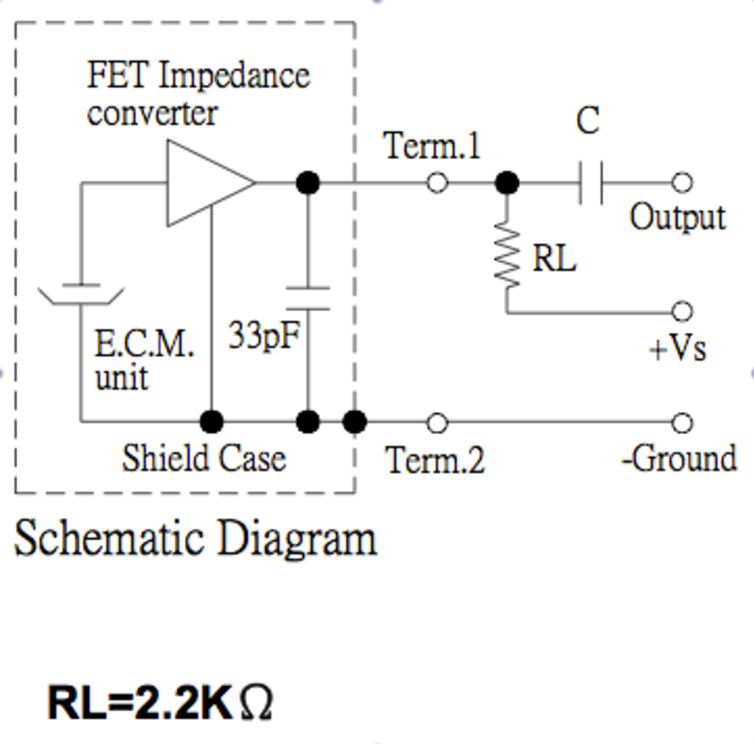
\includegraphics[width=0.7\textwidth]{polarisation_micro.pdf}
\caption{Circuit du microphone}
\label{fig:polarisation du micro}
\end{figure}
Le principe de fonctionnement du micro est que sa membrane extérieure mobile constitue l'armature d'un condensateur chargé en permanence, la deuxième armature étant fixe. Le mouvement de cette membrane, dû aux variations de pression, va modifier la capacité du condensateur, et donc la tension à ses bornes. Le microphone est dit piézoélectrique. Dans notre cas, le microphone est aussi dit "à électret", ce qui signifie qu'il ne nécessite pas d'alimentation pour maintenir le condensateur chargé : le matériau constituant la membrane présente la propriété de conserver une charge électrostatique. Cependant, une alimentation est nécessaire pour polariser le transistor de l'étage de sortie du microphone, au travers de la résistance $R_L$. 

\subsection{Montage amplificateur}
Comme nous l'avons dit précédemment, le signal en sortie de notre micro a une amplitude maximale de \SI{1}{\milli\volt}. La plage des tensions d'entrée de l'ADC va de \SI{0}{\volt} à \SI{3.3}{\volt}, afin d'occuper cette plage le plus largement possible tout en gardant une marge de sécurité par rapport à la saturation de l'ADC, il nous était demandé de traiter notre signal de façon à le centrer sur \SI{1.65}{\volt} et atteindre une valeur crête à crête de \SI{3}{\volt}. Pour cela nous avons utilisé deux étages amplificateurs, respectivement d'un gain de 68 et 22. Nous avons donc utilisé le montage représenté à la figure \ref{fig:etage amplificateur}. 

Calculons d'abord la tension à la sortie du premier étage ($V_{out 1}$), à l'aide du principe de superposition. On considère d'abord la seule source de tension continue, la capacité est alors un circuit ouvert (\ref{eqn:2.1}):
\begin{figure}[htbp]
\centering
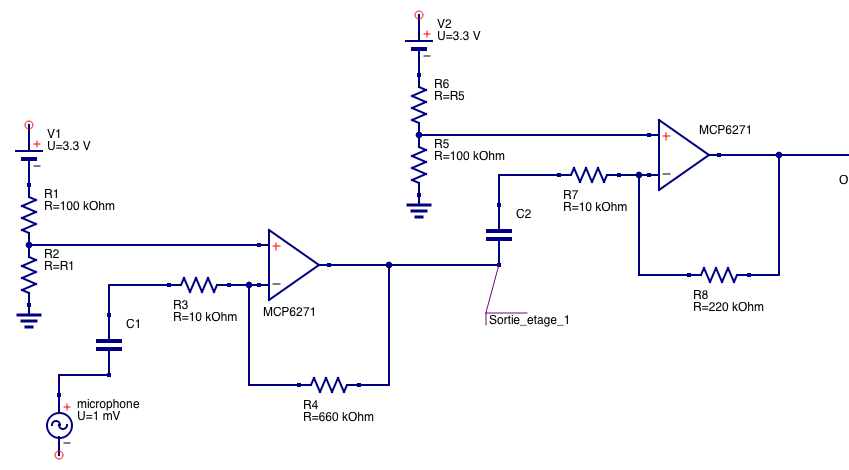
\includegraphics[width=0.7\textwidth]{etage_amplificateur.png}
\caption{Étage amplificateur}
\label{fig:etage amplificateur}
\end{figure}
\begin{equation}
V_{+} = V_{-} = V_{out 1} = \SI{1.65}{\volt}
\label{eqn:2.1}
\end{equation}
Considérons ensuite uniquement la source de tension continue, le circuit est alors un inverseur classique (\ref{eqn:2.2}) : 
\begin{equation}
V_{out 1} = \frac{R_2}{R_1} V_{micro} = 68 V_{in}
\label{eqn:2.2}
\end{equation}
On retrouve la tension en sortie du premier étage en sommant ces deux termes pour finalement obtenir (\ref{eqn:2.3}) :
\begin{equation}
V_{out 1} = \SI{1.65}{\volt} + 68 V_{micro}
\label{eqn:2.3}
\end{equation}

La capacité $C_{2}$ placée entre nos deux étages d'amplification sert à supprimer la composante continue de la tension, la recentrant autour de \SI{0}{\volt}. On évite ainsi de faire saturer notre deuxième ampli-op. Pour le deuxième étage, les calculs sont exactement les mêmes que pour le premier, exception faite du gain du montage inverseur qui vaut 22. On obtient alors notre signal amplifié (\ref{eqn:2.4}) : 
\begin{equation}
V_{out final} = \SI{1.65}{\volt} + 1496 V_{micro}
\label{eqn:2.4}
\end{equation}

Pour être persuadé du bon fonctionnement de notre étage amplificateur, nous avons bien sûr effectué des essais sur celui-ci au départ du générateur de fréquences mis à notre disposition. Les résultats obtenus à l'oscilloscope sont entièrement satisfaisants. 

\subsection{Filtre de garde}
\label{Filtre de garde}
Étant donné que nous allons numériser notre signal, il est nécessaire d'utiliser un filtre de garde pour éviter tout repliement spectral. Quelques spécifications nous étaient données pour ce filtre :
\begin{itemize}
\item Il doit s'agir d'un filtre de Butterworth d'ordre 2
\item L'atténuation maximale des fréquences utiles doit être de 0.99
\item L'atténuation minimale des fréquences filtrées doit être de 0.05.
\end{itemize}
L'amplitude de la réponse en fréquence d'un filtre de Butterworth est donné par l'équation \ref{eqn:butterworth}
\begin{equation}
\vert{H(j\omega)}\vert = \sqrt[]{\frac{1}{1+(\frac{\omega}{\omega_c})^{2n}}}
\label{eqn:butterworth}
\end{equation}
Nous connaissons notre fréquence utile maximale, elle est de \SI{1100}{\hertz}. Si nous injectons cette valeur de $\omega$ dans l'équation, nous pouvons remplacer le terme de gauche par 0.99 et n par 2. On peut alors calculer  l'inconnue restante, $\omega_c$, qui vaut \SI{2972.97}{\hertz}.

Maintenant que nous connaissons la fréquence de coupure de notre filtre, nous pouvons calculer la fréquence à partir de laquelle il faut que l'atténuation soit au minimum de 0.05. On remplace dans l'équation \ref{eqn:butterworth} le module de la réponse en fréquence par 0.05, n par 2 et $\omega_c$ par \SI{2972.97}{\hertz}. On obtient comme valeur de $\omega$ \SI{13.287}{\kilo\hertz}. 

Avec toutes ces informations, nous avons utilisé l'outil "Filter Wizard" d'Analog Devices \footnote{http://www.analog.com/designtools/en/filterwizard} qui nous a permis de designer notre filtre.
\begin{figure}[htbp]
\centering
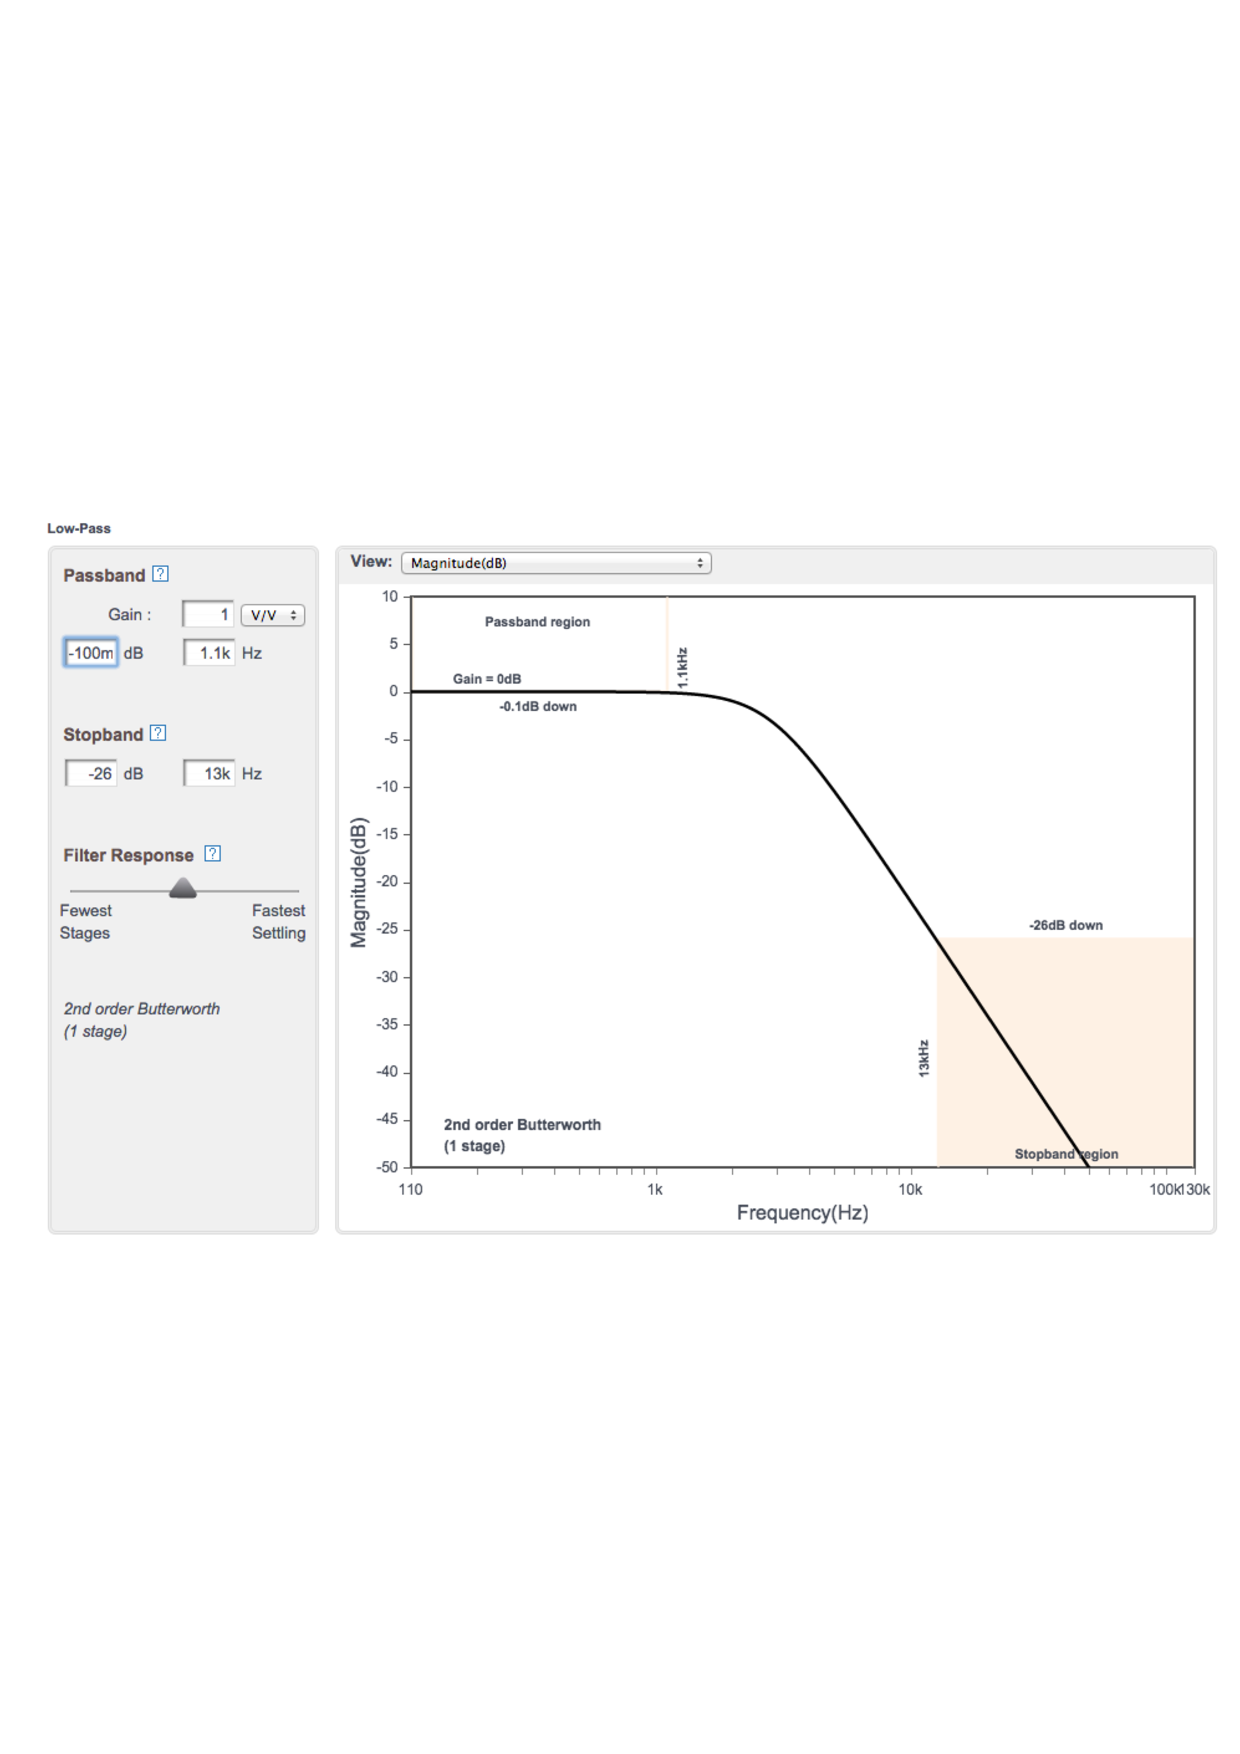
\includegraphics[width=\textwidth]{specs_filtre_analog.pdf}
\caption{L'interface du "Filter Wizard"}
\label{fig:specsAnalogFilter}
\end{figure}
La figure \ref{fig:specsAnalogFilter} montre les spécifications de notre filtre analogique ainsi que l'amplitude de sa réponse en fréquence en fonction de la fréquence. Pour l'implémentation du filtre, Analog nous conseillait un étage Sallen-Key, ce que nous avons fait.
\begin{figure}[htbp]
\centering
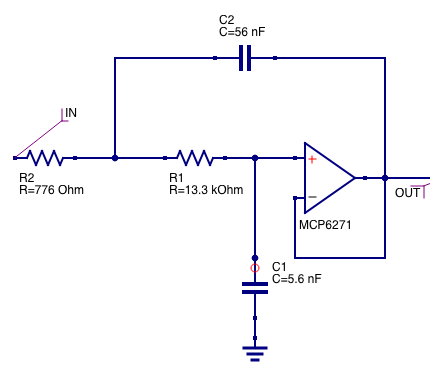
\includegraphics[width = 0.7\textwidth]{filtre_analogique.png}
\caption{Montage de notre filtre analogique}
\label{fig:filtreAnalogique}
\end{figure}
La figure \ref{fig:filtreAnalogique} montre le montage de notre filtre passe-bas. Pour tester notre implémentation, nous lui avons mis en entrée des sinus à différentes fréquences : \SI{900}{\hertz}, \SI{1100}{\hertz}, \SI{13}{\kilo\hertz} (première fréquence atténuée avec un facteur 0.05) et à la fréquence de coupure (\SI{2972.97}{\hertz}). Les résultats sont exposés aux figures \ref{fig:filtreAnalog900Hz}, \ref{fig:filtreAnalog1100Hz}, \ref{fig:filtreAnalog13kHz} et \ref{fig:filtreAnalogFc}. L'entrée est représentée en rouge et la sortie en bleu.
\begin{figure}[htbp]
\centering
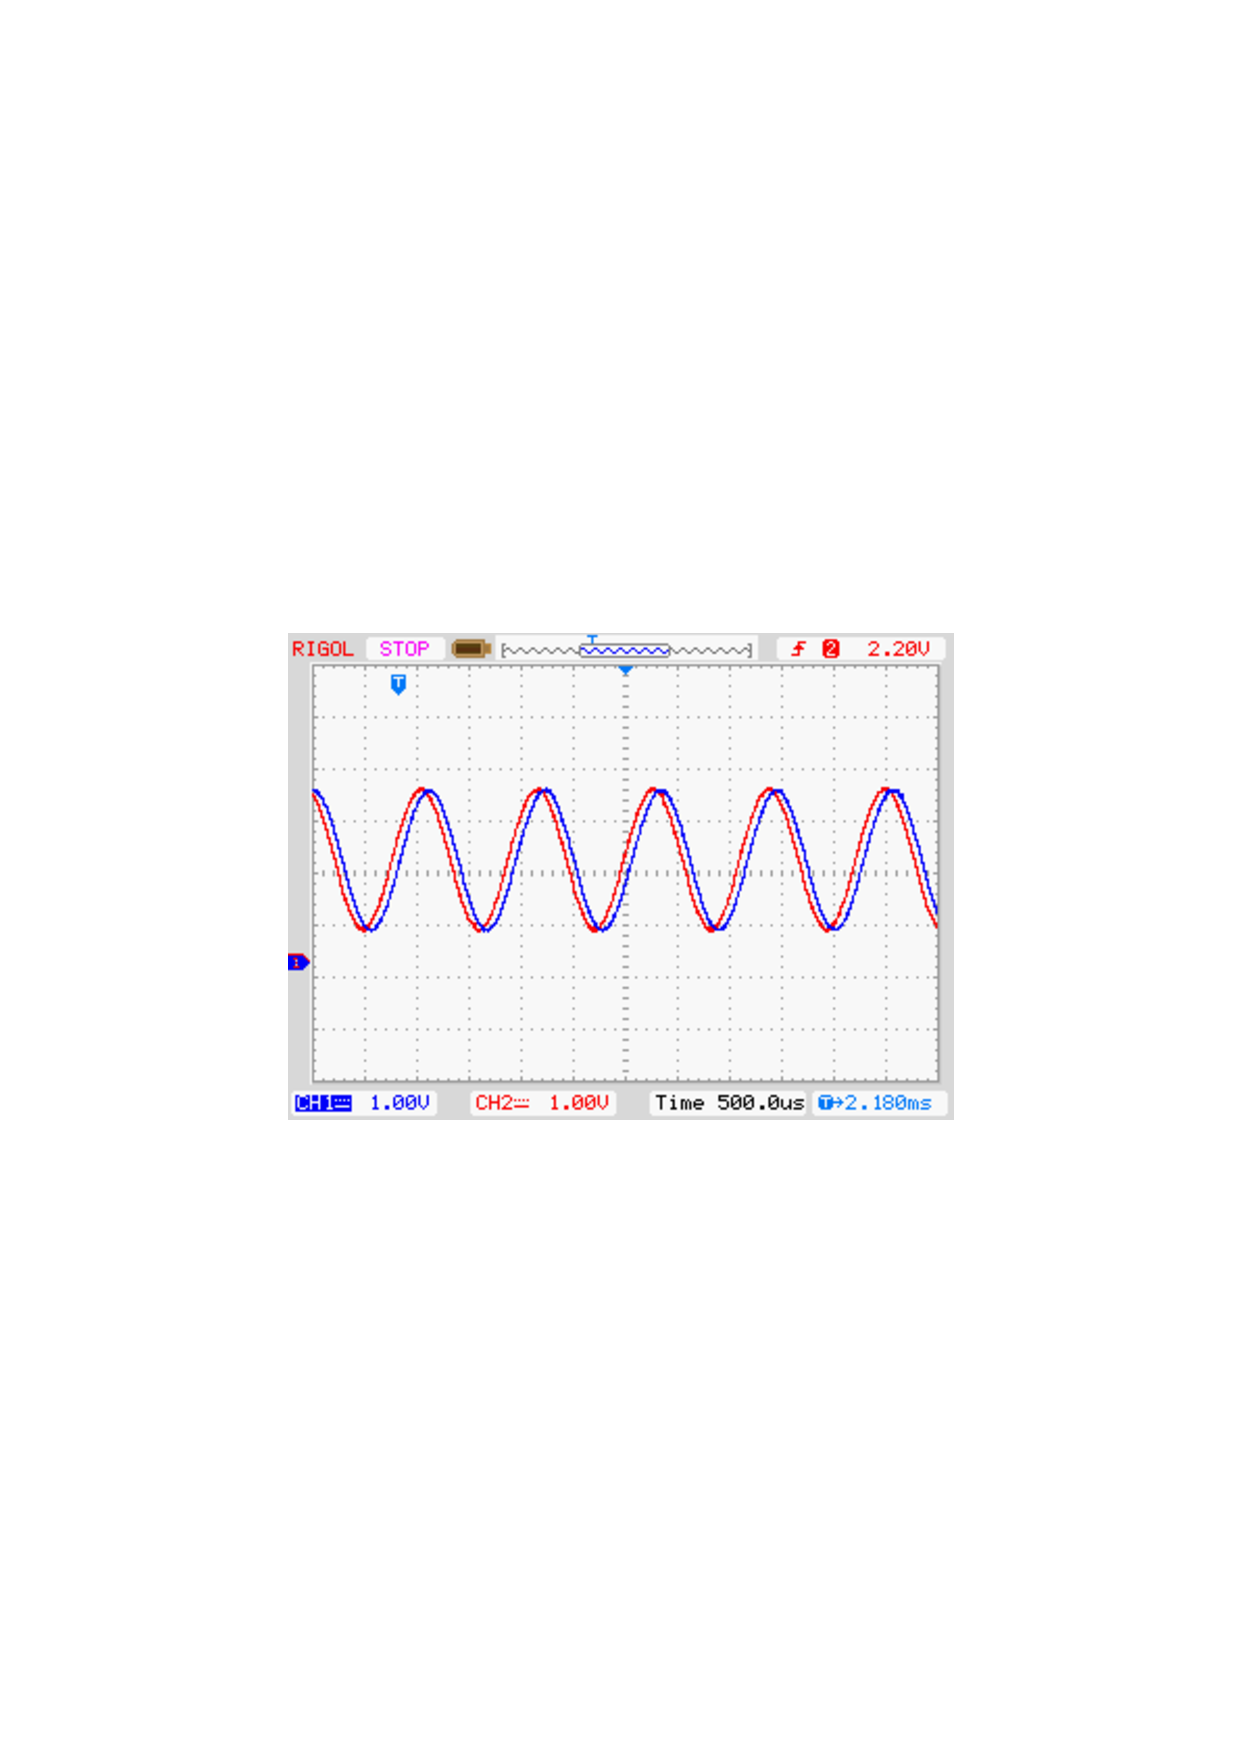
\includegraphics[width = 0.7\textwidth]{filtreAnalog900Hz.pdf}
\caption{\SI{900}{\hertz}}
\label{fig:filtreAnalog900Hz}
\end{figure}
\begin{figure}[htbp]
\centering
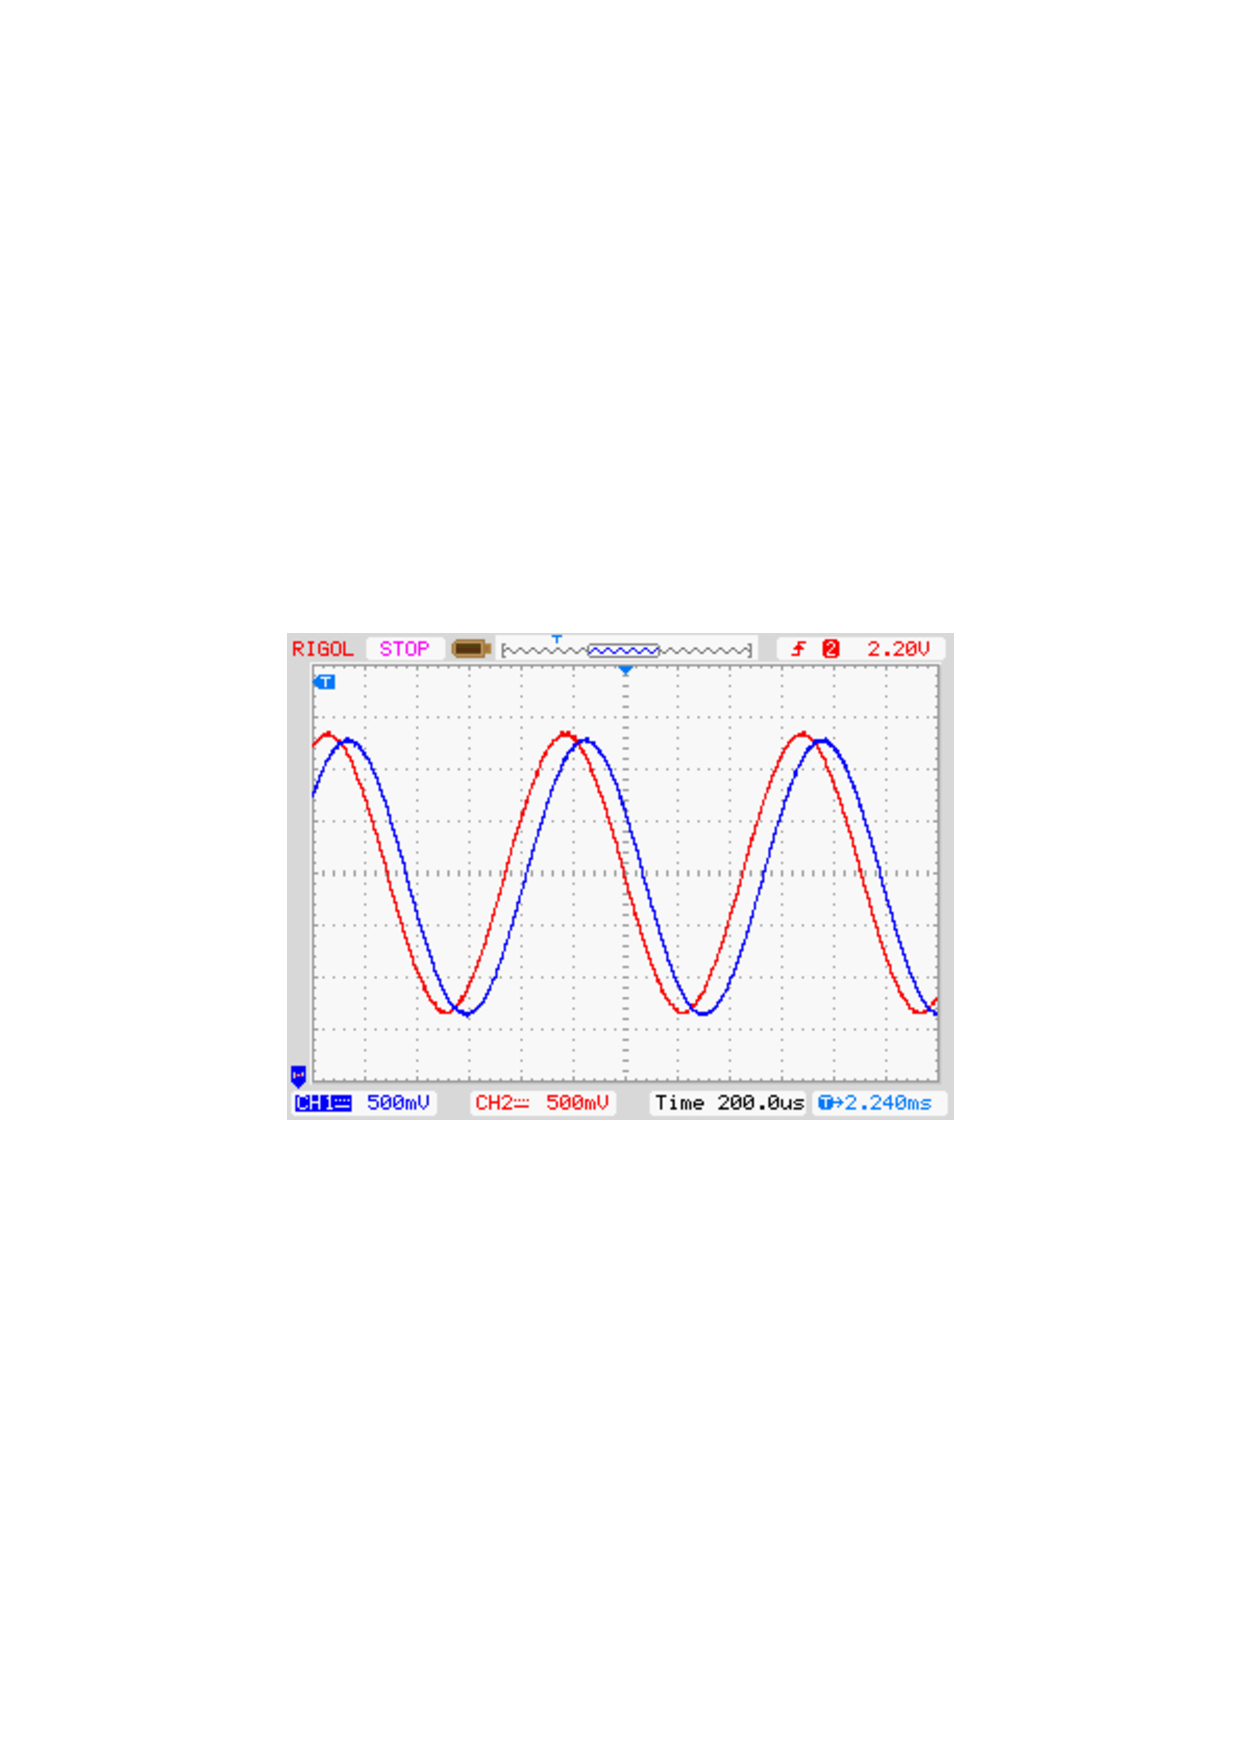
\includegraphics[width = 0.7\textwidth]{filtreAnalog1100Hz.pdf}
\caption{\SI{1100}{\hertz}}
\label{fig:filtreAnalog1100Hz}
\end{figure}
\begin{figure}[htbp]
\centering
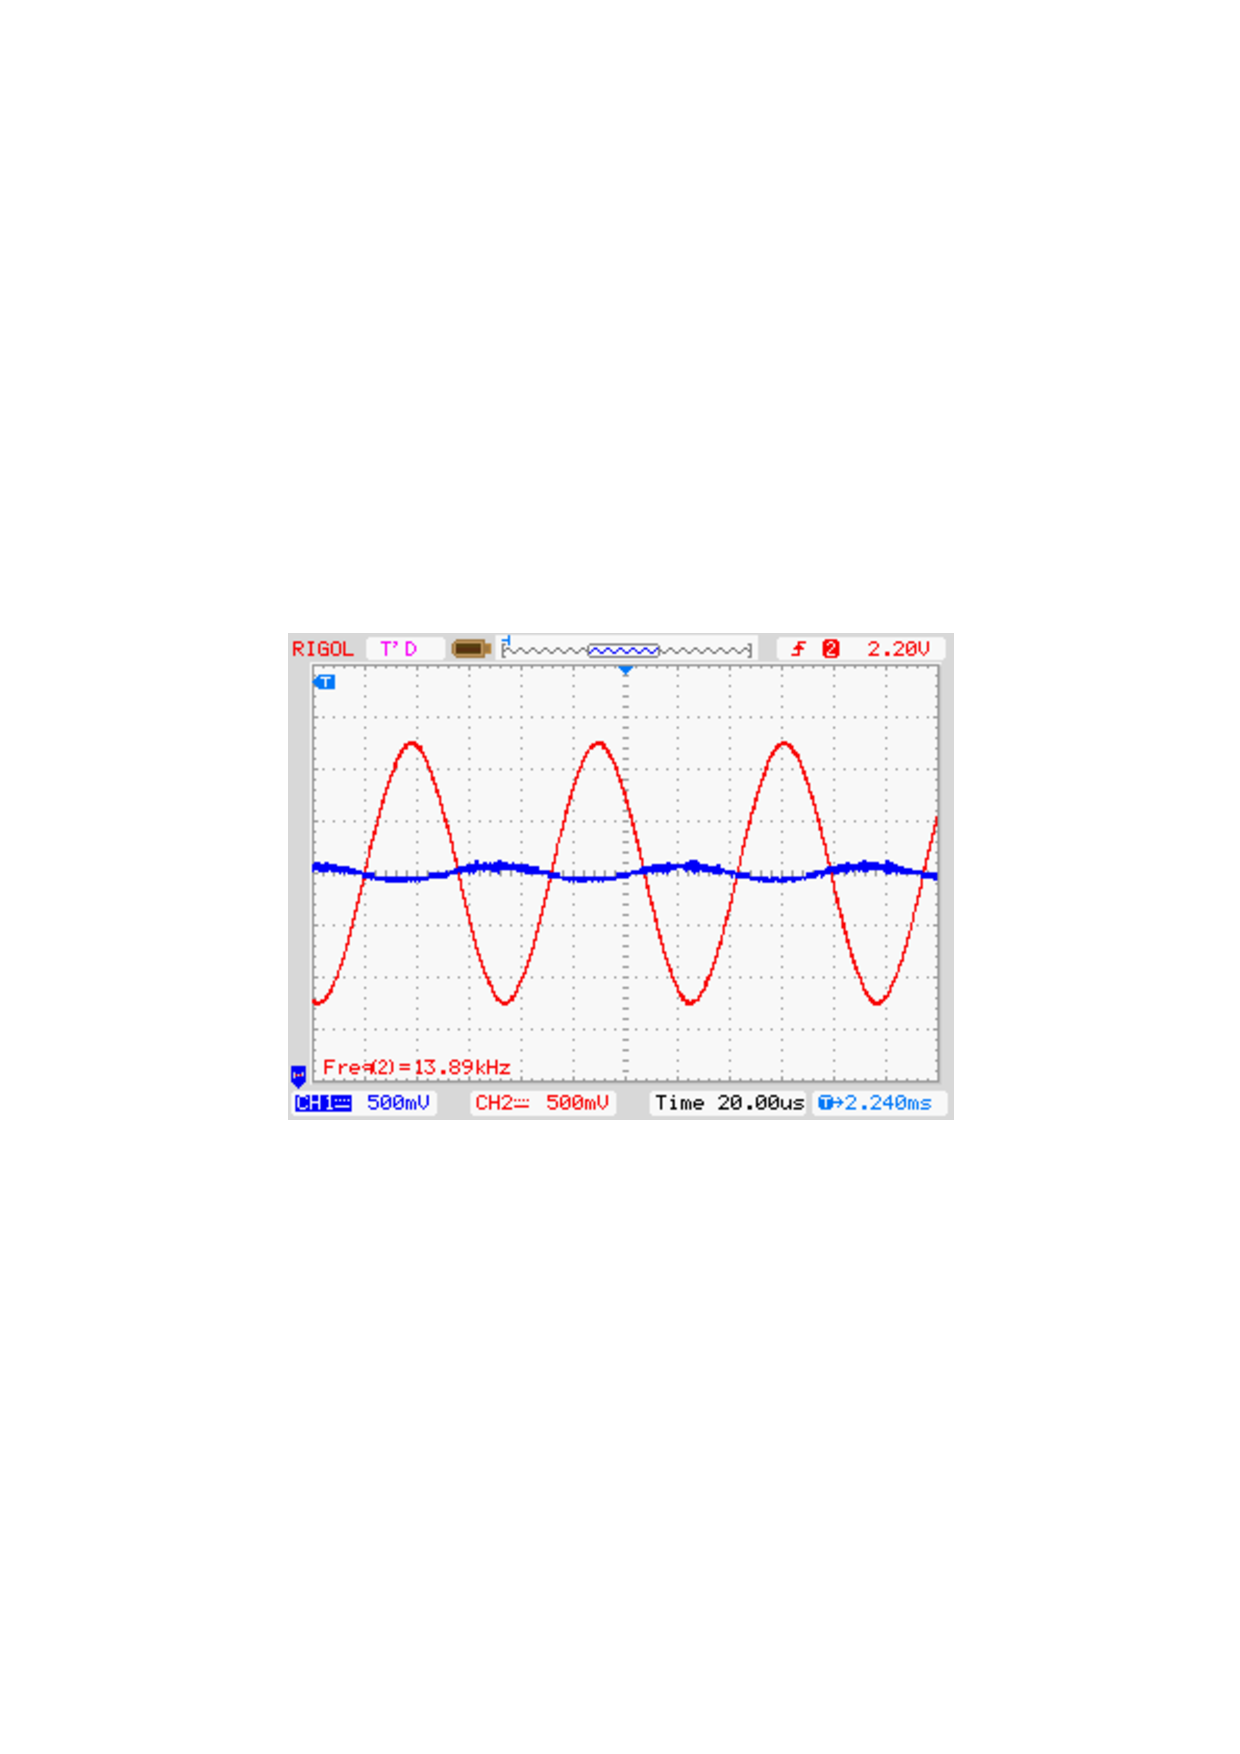
\includegraphics[width = 0.7\textwidth]{filtreAnalog13kHz.pdf}
\caption{\SI{13}{\kilo\hertz}}
\label{fig:filtreAnalog13kHz}
\end{figure}
\begin{figure}[htbp]
\centering
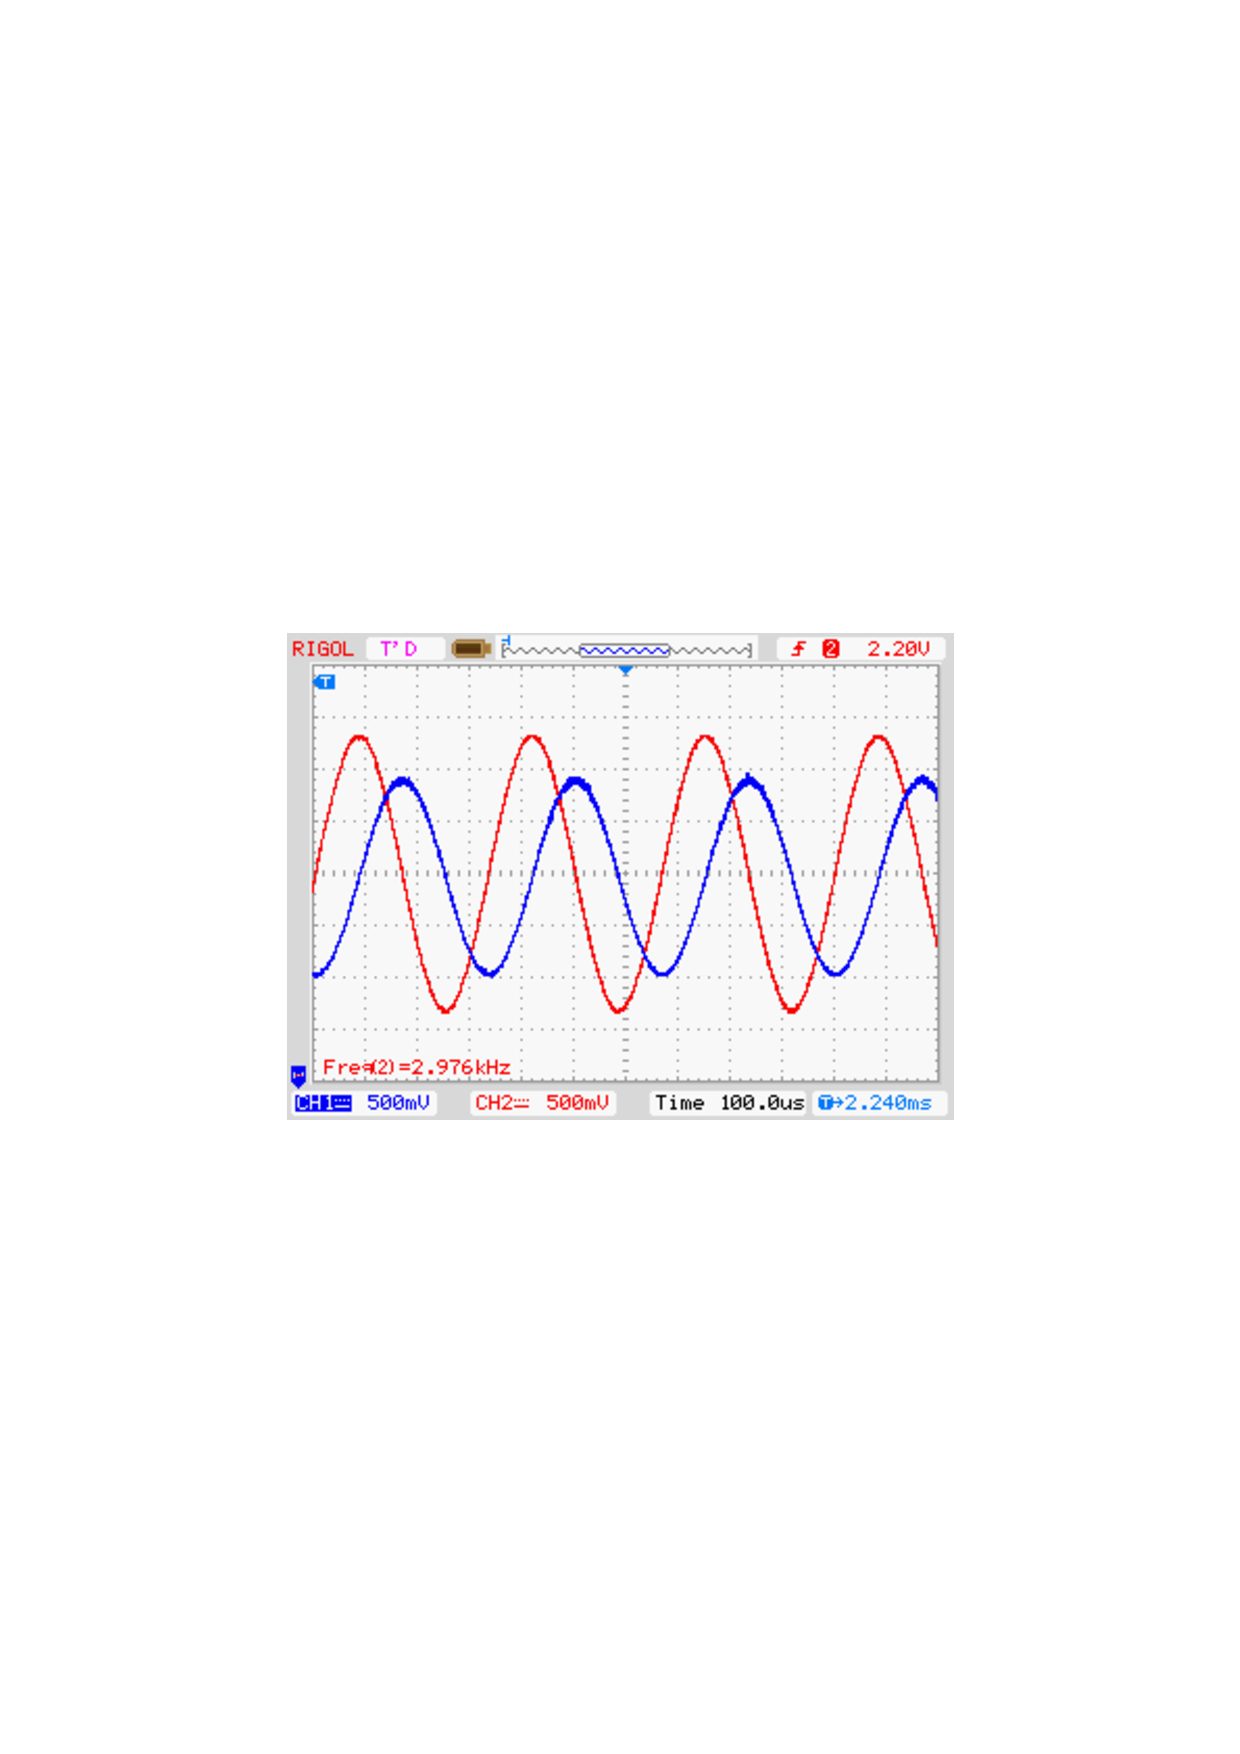
\includegraphics[width = 0.7\textwidth]{filtreAnalogFc.pdf}
\caption{Fréquence de coupure}
\label{fig:filtreAnalogFc}
\end{figure}

\subsection{Le convertisseur analogique-numérique}
Afin que notre microcontrôleur chargé de la communication puisse interpréter les consignes qui lui sont envoyées, il a bien sûr fallu convertir le signal reçu en signal numérique. Pour cela nous avons configuré l'ADC du microcontrôleur communication : c'est la fonction \ilcode{initADC()} qui contient le code correspondant. Ci-dessous nous listons quelques éléments importants de cette configuration :
\begin{itemize}
\item L'ADC fonctionne en mode 12 bits, ce qui est son maximum
\item La tension de référence pour la conversion est la même que la tension d'alimentation
\item L'ADC requiert un certain temps de conversion, la période de conversion de l'ADC est posée à 10 fois la période du microcontrôleur
\item L'ADC commence automatiquement à échantillonner lorsqu'il termine une conversion
\item L'ADC déclenche une conversion à chaque période du timer 3
\item Chaque conversion entraîne une interruption
\end{itemize}
Ce dernier point est particulièrement important, car c'est dans cette interruption que se déroule bon nombre d'opérations cruciales au fonctionnement du robot. La trame sortant de l'ADC y est filtrée par nos filtres numériques, et passe dans le détecteur de crête. Le signal est alors démodulé et envoyé au microcontrôleur chargé du déplacement s'il s'agit bien d'un ordre. 

\subsection{Les filtres numériques et comparateurs}
Une fois notre signal numérisé, il faut encore en extraire la commande, s'il y en a bien une. Pour cela nous devons détecter la présence de nos deux fréquences de modulation : \SI{900}{\hertz} et \SI{1100}{\hertz}. En pratique, on filtre le signal de façon à ce que toutes les autres fréquences soient atténuées et on vient ensuite vérifier si l'amplitude du signal dépasse encore un certain seuil. Ces deux tâches incombent respectivement aux fonctions \ilcode{filterNewSample(unsigned int sample, int returnArray[2])} et \ilcode{peakDetect(int input[2])}.

Pour ce qui est des filtres, ce sont des filtres récursifs du second ordre normalisés. Ils sont décrits par l'équation recursive \ref{eqn:filtre_recursif} que l'on retrouve dans la fonction \ilcode{recurrence(long a1, long a2, long gain,int arrayX[3], long arrayY[3])} ou par le schéma bloc de la figure \ref{fig:filtre_bloc} :
\begin{equation}
y(n) = b_0x(n) + b_1x(n-1) + b_2x(n-2) - a_1y(n-1) - a_2y(n-2)
\label{eqn:filtre_recursif}
\end{equation}
\begin{figure}
\centering
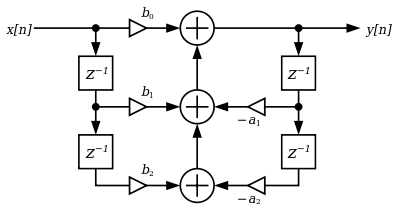
\includegraphics[width=0.7\textwidth]{filtre_bloc.png}
\caption{Schéma bloc d'un filtre numérique du second ordre}
\label{fig:filtre_bloc}
\end{figure}
Nous avons utilisé l'outil \ilcode{fdatool} de Matlab pour trouver les coefficients de nos deux filtres. En donnant comme paramètres au programme les spécifications qui nous étaient imposées, les filtres obtenus étaient composés de quatre sections d'ordre 2. Nous avons commencé par tester ces filtres de manière indépendante du reste du montage et ils fonctionnaient alors très bien. Cependant quand on les plaçait derrière notre ADC, les sorties des filtres n'avaient plus aucun sens. Après un moment, nous nous sommes aperçu que nos filtres étaient tout simplement trop lent : le temps de calcul nécessaire ralentissait le fonctionnement de l'ADC (nous rappelons que le filtrage a lieu dans l'interruption de l'ADC). Pour nous en rendre compte, nous avons flippé un bit sur une des pattes du microcontrôleur dans cette même interruption de l'ADC et nous avons mesuré la fréquence du signal ainsi obtenu à l'oscilloscope. Si l'ADC arrive à fonctionner à la fréquence d'échantillonnage $f_s$  prévue, que nous avions au départ fixée à \SI{27}{\kilo\hertz} en accord avec les calculs du point \ref{Filtre de garde}, la fréquence mesurée doit être égale à $\frac{f_s}{2}$ (le bit est flippé à chaque interruption de l'ADC, une période représente donc deux périodes de l'ADC). Nous avons donc tenté de rendre nos filtres plus rapides en modifiant le code, par exemple en remplaçant tous les nombres de type \ilcode{float} par des \ilcode{int}. Mais au final, nous avons du diminuer notre fréquence d'échantillonnage à \SI{20}{\kilo\hertz} et n'utiliser que la première section de nos filtres. Leurs performances en sont diminuées, mais ils restent assez efficace. Les courbes de Bode du filtre à une seule section centré autour de \SI{900}{\hertz} que nous utilisons pour finir sont données à la figure \ref{fig:filtre_1section}.
\begin{figure}
\centering
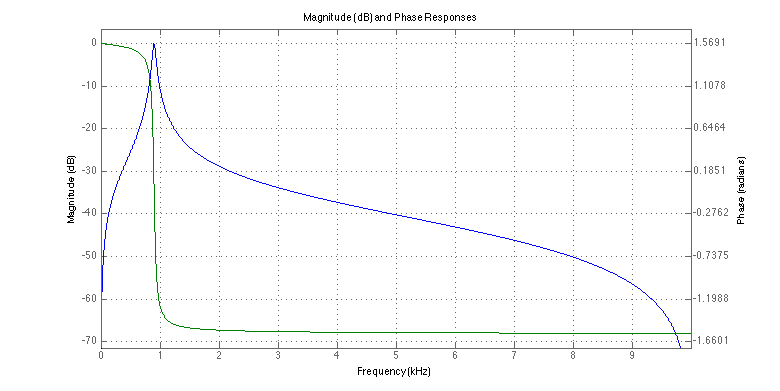
\includegraphics[width=\textwidth]{filtre_1section.png}
\caption{Courbes de Bode du filtre numérique centré autour de \SI{900}{\hertz}}
\label{fig:filtre_1section}
\end{figure}

Derrière les filtres numériques, le signal passe dans deux comparateurs chargés de détecter la présence de \SI{900}{\hertz} ou \SI{1100}{\hertz}. Pour cela, le microcontrôleur garde en mémoire un bloc du signal correspondant à une période de \SI{1/900}{\second} ou \SI{1/1100}{\second} et trouve le maximum sur ce bloc. Si ce maximum dépasse un certain seuil, la fréquence correspondante est présente. Ces informations sont alors transmises à la fonction \ilcode{fskDetector(int detLow, int detHigh)} qui va mettre en forme la trame détectée.